%!TEX root = draft.tex
%\newcommand{\seqPQ}{\mathsf{SeqPQ}}

\section{CRDT Implementations}
\label{sec:CRDT implementations}

A distributed system contains multiple objects, and each objects is replicated on each replica. Each object has a type, which contains its method and data type. A client of a replica interact with the objects by calling the method and then obtaining the return value. Here we do not bound the number of replica identifiers and objects.

Let $\mathbb{OBJ}$ be the set of objects and $\mathbb{R}$ be the set of replica identifiers. We consider a finite set $\mathbb{M}$ of method names; and a possibly infinite set $\mathbb{D}$ of arguments and return values, the data domain. Each data type $t = (M,D)$ has a set $M \subseteq \mathbb{M}$ of methods and a data domain $D \subseteq \mathbb{D}$. Finally we have a infinite set $\mathbb{OID}$ of operation identifiers, corresponding to each individual operation performed on the CRDT throughout an execution.

Without loss of generality we will consider that the methods in $\mathbb{M}$ can be separated in two disjoint sets of methods: $\mathbb{Q}$ query methods that has no influence on the ``abstract state'' and normally returns an observation of the ``abstract state'' , and $\mathbb{U}$ update methods that has influence on the ``abstract state''. Note that some update operation can also need to read the ``abstract state''. For example, a $add(a,b)$ operation is an operation of distributed list which intends to put item $a$ immediately after item $b$. This operation implicitly requires that item $b$ is already in list.

$\mathit{Optimistic \ replication \ algorithms}$ is a type of distributed algorithms where each client contains a copy of data structure; a client operations takes effect instantly at its replica without any synchronization, and then broadcast to other replicas and got applied. Convergent or Commutative Replicated Data Types (CRDTs) is a typical kinds of optimistic replication algorithms. In this section, we will introduce CRDT algorithms and their formation.

In practice, there are two kinds of CRDT implementations: state-based CRDT and operation-based CRDT. In state-based CRDT, an update operation will send the modified local state into other replicas. The state-based PN-counter is an example of state-based CRDT algorithms and is shown below. Keyword $\mathit{payload}$ indicate the local state, and keyword $\mathit{initial}$ specifies the initial value of local state. Function $\mathit{myID}()$ returns the current replica identifier, and $\mathit{reps}()$ returns the number of replicas of the distributed system. Vector $P$ (resp., $N$) is a vector such that $P[i]$ (resp., $N[i]$) is the number of increase that is generated by replica $i$ and is observed by current replica. This algorithm assumes that the set of replica is already known and is fixed.

Method $\mathit{inc}$ increase the counter by $1$, method $\mathit{dec}$ decrease the counter by $1$, and method $\mathit{read}$ returns the current counter value. Assume the replica identifier of current replica is $r$. When the current replica does $\mathit{inc}$, it modify $P[r]$ into $P[r]+1$. When the current replica does $\mathit{dec}$, it modify $N[r]$ into $N[r]+1$. When the current replica does $\mathit{read}$, it returns $\Sigma_{i}^{n} P[i] - \Sigma_{i}^{n} N[i]$. When the current replica receive a message of modified payload $Z$, it uses function $\mathit{merge}()$ to update the current local state. $\mathit{merge}$ takes the maximum of each replica in the vector.

\renewcommand{\algorithmcfname}{CRDT Implementation}
\noindent
%\begin{minipage}{.5\textwidth}
\noindent\begin{algorithm}[H]
$\mathit{payload}$ integer[$\mathit{reps}$()] P, integer[$\mathit{reps}$()] N; \\
$\mathit{initial}$ [0,\ldots,0],[0,\ldots,0]; \\

$\mathit{inc}()$ \\
%\ \ \ \ let \ g = myID();\\
\ \ \ \ P[$\mathit{myID}$()] = P[$\mathit{myID}$()] + 1; \\

$\mathit{dec}()$ \\
%\ \ \ \ let \ g = myID();\\
\ \ \ \ N[$\mathit{myID}$()] = N[$\mathit{myID}$()] + 1; \\

$\mathit{read}()$ \\
\ \ \ \ \KwRet $\Sigma_{i}^{n} P[i] - \Sigma_{i}^{n} N[i]$; \\

$\mathit{merge}(Z)$ \\
\ \ \ \ $\forall i$, $P[i] = \mathit{max}(P[i],Z.P[i])$; \\
\ \ \ \ $\forall i$, $N[i] = \mathit{max}(N[i],Z.N[i])$; \\
\caption{State-based PN-counter}
\label{Method1}
\end{algorithm}

In operation-based CRDT, an update operation will send a description of this operation into other replica. Here we take a more complex algorithm, replicated growable array (RGA), as an example of operation-based CRDT and it is shown below.

\renewcommand{\algorithmcfname}{CRDT Implementation}
\noindent
%\begin{minipage}{.5\textwidth}
\noindent\begin{algorithm}[H]
$\mathit{payload}$ TI-tree N, set T; \\
$\mathit{initial}$ $\emptyset$,$\emptyset$; \\

$add(a,b)$ \\
\ \ $\mathit{atSource}$: \\
\ \ \ \ $\mathit{pre}$: \ $b = \circ \vee ( b \neq \circ \wedge (b,\_,\_) \in N \wedge b \notin T)$ \\

%\ \ \ \ \If {$N = \emptyset$}
%    { \ \ \ \ let \ $ts_a$ = (myID(),1); \\ }
%\ \ \ \ \Else
%    {\ \ \ \ let \ $ts_a$ = (myID(),$\mathit{max}\{ c' \vert (\_,(\_,c'),\_) \in N \} +1$); \\ }

%\ \ \ \ \If {$b = \circ$}
%    { \ \ \ \ let \ $ts_b$ = (0,0); \\ }
%\ \ \ \ \Else
%    { \ \ \ \ let \ $ts_b$ be time-stamp of $b$ in $N$; \\ }

\ \ \ \ let \ $ts_a$ = ($N = \emptyset$) ? (1,$\mathit{myID}$()) ! ($\mathit{max}\{ c' \vert (\_,(\_,c'),\_) \in N \} +1$,$\mathit{myID}$()); \\
\ \ \ \ let \ $ts_b$ = ($b = \circ$) ? (0,$r_0$) ! (the time-stamp of $b$ in $N$); \\

\ \ $\mathit{downstream}(a,ts_a,ts_b)$: \\
\ \ \ \ $\mathit{pre}$: \ $b = \circ \vee ( b \neq \circ \wedge (b,ts_b,\_) \in N)$ \\

\ \ \ \ $N = N \cup \{ (a,ts_a,ts_b) \}$.


$rem(a)$ \\
\ \ $\mathit{atSource}$: \\
\ \ \ \ $\mathit{pre}$: \ $a \neq \circ \wedge (a,\_,\_) \in N \wedge a \notin T$ \\

\ \ $\mathit{downstream}(a)$: $\mathit{pre}$ \ $a \neq \circ \wedge (a,\_,\_) \in N)$

\ \ \ \ $T = T \cup \{ a \}$.

$read()$ \\
\ \ \ \ \KwRet $\mathit{trans}(N,T)$; \\

\caption{RGA}
\label{Method1}
\end{algorithm}

Each update operation of operation-based CRDT ie executed with two phases: Its first phase, marked $\mathit{atSource}$, is local to the current replica. It is enabled if its (optional) pre-condition, marked $\mathit{pre}$, is true currently in local state. It generates the information to be delivered, which is the argument of $\mathit{downstream}$. Its second phase, marked $\mathit{downstream}$, executed immediate after the current replica, and asynchronously at other replica when they receive the message of this operation. It is enabled if its (optional) pre-condition is true.

In RGA algorithm, a replica store the list as a timestamp insertion tree (TI-tree) $N$, and stores the deleted items in tombstone $T$. A TI-tree $N$ is a set of tuples $(a,t,p)$, where $a$ is a item, $t$ is its unique time-stamp, and $p$ is the time-stamp of its ``parent'' node. Each time-stamp is a tuple $(c,r)$ with $c \in \mathbb{N}$ and $r \in \mathbb{R}$. A order $<_{\mathit{ts}}$ between time-stamps is defined, such that $(c_1,r_1) <_{\mathit{ts}} (c_2,r_2)$, if $c_1 < c_2 \vee (c_1 = c_2 \wedge r_1 <_r r_2)$, where $<_r$ is a total-order over $\mathbb{R}$. There is a pre-existed item $\circ$ of TI-tree with time stamp $(0,r_0)$, which are considered as the root of the tree. Each element of $N$ should have unique item and time stamp, and the elements of $N$ are required to form a tree by following the parent field. The tombstone $T$ is a set of items and records items been removed from the list.

Method $\mathit{add}(a,b)$ intends to add item $a$ into the list immediately after a existing item $b$. Method $\mathit{rem}(a)$ removes $a$ from the list. Method $\mathit{read}$ returns the current list content. When the current replica does $\mathit{add}(a,b)$, it generate a tuple $(a,ts_a,ts_b)$ and put it into $N$. Here $ts_b$ is the time-stamp of $b$, and $ts_a$ is a new time-stamp that is larger than any time stamp in $N$. When the current replica does $\mathit{rem}(a)$, it put $a$ into tombstone. When the current replica does $\mathit{read}$, it uses function $\mathit{trans}(N,T)$ to return the list seen by the current replica, which is a sequences obtained by traversing $N$ in prefix order (children are visited in decreasing time-stamp order) and keeping only items that are not in $T$.


Multi-value register is also a common-used data structures and its sequential specification (seen in the next section) is much different from that of the previous two examples. A state-based multi-value register algorithm is shown below.


\renewcommand{\algorithmcfname}{CRDT Implementation}
\noindent
%\begin{minipage}{.5\textwidth}
\noindent\begin{algorithm}[H]
$\mathit{payload}$ $S \subseteq D \times \mathbb{N}^{\mathit{reps}()}$; \\
$\mathit{initial}$ $\emptyset$; \\

$\mathit{write}(a)$ \\
\ \ \ \ let \ g = $\mathit{myID}$(); \\
\ \ \ \ let $\mathcal{V} = \{ V \vert \exists x, (x,V) \in S \}$; \\
\ \ \ \ let $V' = [ \mathit{max}_{V \in \mathcal{V}} V[j] ]_{j \neq g}$; \\
\ \ \ \ let $V'[g] = (\mathit{max}_{V \in \mathcal{V}} V[g]) + 1$; \\
\ \ \ \ $S = (a,V')$; \\

$\mathit{read}()$ \\
\ \ \ \ \KwRet $S' = \{ a \vert (a,\_) \in S \}$; \\

$\mathit{merge}(Z)$ \\
\ \ \ \ let $A' = \{ (x,V) \in S \vert \forall (x',V') \in Z.S, \exists i, V[i] \geq V'[i] \}$; \\
\ \ \ \ let $B' = \{ (x,V) \in Z.S \vert \forall (x',V') \in S, \exists i, V[i] \geq V'[i] \}$; \\
\ \ \ \ $S = A' \cup B'$; \\
\caption{state-based multi-value register}
\label{Method1}
\end{algorithm}

Each replica stores a set $S$ of items such that each item can not dominate other items. To do conflict resolution, we associate each item $a$ in $S$ with a version vector $V$. We say version vector $V$ dominates version vector $V'$, if $\forall i$, $V[i] > V'[i]$.

Method $\mathit{write}(a)$ intends to write $a$ into register. Method $\mathit{read}$ returns the current register content. When the current replica does $\mathit{write}(a)$, it generates a new version vector that dominates all previous ones in $S$. When the current replica does $\mathit{read}$, it returns the set of items in $S$. When the current replica receive a message of modified payload $Z$, we takes the union of every items in $S$ and $Z.S$ whose version vector is not dominated by that of an item in the other set. This algorithm assumes that the set of replica is already known and is fixed.


To enable formally verification of CRDT algorithms, it is necessary to give formal definition of CRDT-algorithms. Let $\mathbb{MSG}$ be the set of message contents, such as $inc$ of state-based PN-counter, or $(a,ts_a,ts_b)$ of RGA. Then, CRDT implementations are defined as follows, where operations and receiving messages are defined as functions.

\begin{definition}[CRDT implementations]
\label{definition:CRDT implementations}
A CRDT implementation for a type $t = (M,D)$ is a tuple $I_t(r) = (\Sigma, \Sigma_0, \mathit{Msg}, \mathit{do},\mathit{receive})$. Here $r \in \mathbb{R}$, $\Sigma_0 \subseteq \Sigma$, $\mathit{Msg} \subseteq \mathbb{MSG}$, $\mathit{do}:\Sigma \times M \times D \rightarrow \Sigma \times D \times (\mathit{Msg} \cup \{ \emptyset \} )$, and $\mathit{receive}: \Sigma \times \mathit{Msg} \rightarrow \Sigma$.
\end{definition}

Here $\Sigma$ is the set of local states and $\Sigma_0$ is the set of initial state. For example, in state-based PN-counter, since there are many possibility of total number of replicas, $\Sigma_0$ is a set of more than one elements. $r$ is the replica identifier of current replica. The reason of containing $r$ in the definition of CRDT implementations is that, some algorithms need the current replica identifier to generate time-stamp. When the current local state is $\sigma$ and the client intends to perform a operation of method $m$ with argument $a$, a $\mathit{do}$ action is launched, which update the local states, returns a value, and possibly generate messages. A $\mathit{do}$ action of update method will generate messages, while a $\mathit{do}$ action of query method will not generate message. When this replica receives a message of other replica, a $\mathit{receive}$ action will be launched, which updates the current local states according to the message. If a operation has no arguments or return value, or does not generate message, then we can safely omit the corresponding tuples in $\mathit{do}$ actions.

The following is an example of formal definition of state-based PN-counter. The formal definition of more CRDT implementations are given in Appendix \ref{sec:appendix definitions of section CRDT implementations and its semantics}. Here we denote by $f[i:j]$ the function that has the same value as $f$ everywhere, except for $i$, where it has the value $j$. Since each operation is executed without synchronization, it is not hard to obtain formal definition from informal algorithms.

\begin{example}[state-based PN-counter]
\label{definition:state-based PN-counter}
$I_t(r) = (\Sigma, \sigma_0, \mathit{Msg}, \mathit{do},\mathit{receive})$, where

\begin{itemize}
\setlength{\itemsep}{0.5pt}
\item[-] $\Sigma = \{ (P,N) \vert$, $P$ and $N$ are vector of integers with same length $\}$. $\Sigma_0 = \{ (P_0,N_0) \vert (P_0,N_0) \in \Sigma$, $P_0$ and $N_0$ maps each index into $0 \}$.

\item[-] $\mathit{Msg} = \Sigma$.

\item[-] $\mathit{do}((P,N),\mathit{inc}) = (P[r:P[r]+1],N),(P[r:P[r]+1],N))$,

\item[-] $\mathit{do}((P,N),\mathit{dec}) = (P,N[r:N[r]+1]),(P,N[r:N[r]+1])$,

\item[-] $\mathit{receive}((P,N),(P',N')) = (\lambda s. \mathit{max}\{  P[s], N'[s] \}, \mathit{max}\{  N[s], N'[s] \},)$,
\end{itemize}
\end{example}





















\section{Distributed Linearizability}
\label{sec:distributed-lin}

In this section, we propose a framework to specify the expected outcome in a linearizable approach, without referring to implementation details.



\subsection{Histories}
\label{subsec:histories}

We define our specification on histories, which are abstract version of detailed executions and does not contain implementation details such as message delivery. Histories are used to capture the notion of client-observable effects (operations), as well as their order in each replica, and their visibility relation.

Let us introduce the notion of operations. A operation label $m(a) \Rightarrow b$ with $m \in \mathbb{M}$ and $a,b \in \mathbb{D}$ is the user-observable behavior of an operation, which indicates that this operation calls method $m$ with argument $a$ and its return value is $b$. An operation is defined to be a tuple $(\ell,i,x)$, where $\ell$ is a operation label, $i \in \mathbb{OID}$ is a unique operation identifier, and $x \in \mathbb{OBJ}$ is the objects of this operation. Let $\mathbb{OP}$ be the set of operations. For operation label $m(a) \Rightarrow b$, when the argument (resp., return value) is not used, we write $m()\Rightarrow b$ (resp., $m(a)$) instead for short.

With the notion of operations, we can now define histories.

\begin{definition}[histories]
\label{definition:histories}
A history is a tuple of the form $(\mathit{Op},\mathit{ro},\mathit{vis})$ .Here $\mathit{Op} \subseteq \mathbb{OP}$ is a set of operations; $\mathit{ro} \subseteq \mathit{Op} \times \mathit{Op}$ is the replica order, which is a union of transitive, irreflexive and total orders over $\mathit{Op}$; $\mathit{vis} \subseteq \mathit{Op} \times \mathit{Op}$ is the visibility order, which is acyclic and relates operations of same object. We also require that $\mathit{ro} \subseteq \mathit{vis}$.
\end{definition}

$(o_1,o_2) \in \mathit{ro}$ represents that $o_1$ and $o_2$ are of same replica and the time point of $o_1$ is before that of $o_2$. $(o_1,o_2) \in \mathit{vis}$ means that $o_2$ is aware of $o_1$. In detailed execution, this means that some message carrying the effect of $o_1$ has already been delivered into replica of $o_2$. In state-based CRDT implementation, this message contains some state aware of $o_1$, while in operation-based CRDT implementation, this message is the message of $o_1$.





\subsection{Sequential Specification}
\label{subsec:sequential specification}

A sequential specification intends to propose a linearizable explanation for distributed objects.

For objects of simple types, a sequential specification is a set of operation sequences. Normally, the sequential specification is defined by the pre-condition and post-conditions. For example, the following is the sequential specification for distributed counter, and is given as a set of transition rules between states. Each state contains a integer value. Transition rule $\{ \mathit{state} = i \}$ $(\mathit{inc},\_,\_)$ $\{ \mathit{state} = i+1 \}$ indicates that $\mathit{inc}$ will increase the state by $1$. Since this rule does not use operation identifier and object, it is safe to shorten this rule into $\{ \mathit{state} = i \}$ $\mathit{inc}$ $\{ \mathit{state} = i+1 \}$. Similarly for $\mathit{dec}$ and $\mathit{read}$ operations. We write $s {\xrightarrow{o}} s'$ to indicate one step of $o$ transition between states $s$ and $s'$ that satisfies some transition rule.

A sequence $(\ell_1,i_1,x) \cdot \ldots \cdot (\ell_k,i_k,x)$ is in sequential specification $\mathit{counter}_s$, if there exists state $s_k$, such that $s_0 {\xrightarrow{(\ell_1,i_1,x)}} \ldots {\xrightarrow{(\ell_k,i_k,x)}} s_k$, and $s_0$ is the initial state. For example, it is easy to see that $(\mathit{inc},\mathit{id}_1,x) \cdot (\mathit{inc},\mathit{id}_2,x) \cdot (\mathit{dec},\mathit{id}_3,x) \cdot (\mathit{read} \Rightarrow 1,\mathit{id}_4,x) \in \mathit{counter}_s$. Note that operations of one sequence of $\mathit{counter}_s$ must be of a same object. We also implicitly assume that each operation has a unique operation identifier.


\begin{example}[sequential specification of counter]
\label{definition:sequential specification of counter}
The sequential specification $\mathit{counter}_s$ of counter is given as follows: Let $\mathit{state}$ be a integer with initial value $0$.

\begin{itemize}
\setlength{\itemsep}{0.5pt}
\item[-] $\{ \mathit{state} = i \}$ $\mathit{inc}$ $\{ \mathit{state} = i+1 \}$.
\item[-] $\{ \mathit{state} = i \}$ $\mathit{dec}$ $\{ \mathit{state} = i-1 \}$.
\item[-] $\{ \mathit{state} = i \}$ $(\mathit{read}() \Rightarrow i)$ $\{ \mathit{state} = i \}$.
\end{itemize}
\end{example}

However, for objects of some types which are designed only for distributed system, such as multi-value register and OR-set, sequential specification in above style seems insufficient (we explain this in the next subsection). To solve this problem, in the transition rules of sequential specification, for some operations, we give them a additional argument which is a set of operation identifiers. Such additional argument essentially represents the operations visible to this operation. We use the sequential specification of multi-value register as example to explain this, which is shown below.

Each state contains a set of tuples $(a,\mathit{id},f)$, where $a$ is item, $\mathit{id}$ is the operation identifier of the operation that put this tuple, and $f$ indicates whether this item is logically removed or not. Given a state $S$, a $(write(a),\mathit{id},x)$ operation with argument $S_1$, the resulting state is obtained by marking all items in $S$ with $S_1$ identifiers into $\mathit{false}$, and then insert $(a,id,\mathit{true})$ into $S$. A $\mathit{read}$ operation returns value with flag $\mathit{true}$ in state.


\begin{example}[sequential specification of multi-value register]
\label{definition:sequential specification of multi-value register}
The sequential specification $\mathit{MVReg}_s$ of multi-value register is given as follows: Let $\mathit{state}$ be a set and each its element $(a,\mathit{id},f)$ is a tuple of a data $a$, a operation identifier $\mathit{id} \in \mathbb{O}$, and a flag $f \in \{ \mathit{true},\mathit{false} \}$.
\begin{itemize}
\setlength{\itemsep}{0.5pt}
\item[-] $\{ \mathit{state} = S \}$ $((write(a),\mathit{id},x),S_1)$ $\{ \mathit{state} = S[(b,\mathit{id}_1) \in S_2 : \mathit{false}]
\cup
\{ (a,id,\mathit{true}) \}
\}$. Here $S_2 = \{ (b,\mathit{id}_1) \vert (b,\mathit{id}_1,\mathit{true}) \in S \wedge id \in S_1 \}$.
\item[-] $\{ \mathit{state} = S \wedge S_1 = \{ a \vert (a,\_,\mathit{true}) \in S \} \}$ $read() \Rightarrow S_1$ $\{ \mathit{state} = S \}$.
\end{itemize}
\end{example} 

Based on above intuition, let us introduce the notion of sequential specification. Let specification alphabet $\mathbb{A} = \mathbb{OP} \cup \{ (o,s) \vert o \in \mathbb{OP}, s \subseteq \mathbb{OID} \}$. Then, a sequential specification of CRDT is defined as a set of sequences over specification alphabets $\mathbb{A}$. 

%\gp{We should add the specifications (even non-deterministic here.)}
\begin{definition}[Sequential Specification]
\label{definition:sequential specification}
A sequential specification is a set of strings over specification alphabet $\mathbb{A}$. 
\end{definition} 

The methods that needs additional arguments, such as $\mathit{write}$ method of multi-value register and $\mathit{rem}$ method of OR-set, is called special methods of that specification. Given a sequential specification  A sequential specification is $\mathit{deterministic}$, if in each of its rules, from each state with each operation, there is at most one resulting state. Otherwise, it is a $\mathit{nondeterministic}$ specification. In the following we will introduce several types and their sequential specifications. $\mathit{list}_s^{\mathit{ab}}$, a version of list specification, is nondeterministic, while all other sequential specifications are deterministic.


\begin{example}[set and its sequential specification]
\label{definition:sequential specification of set}
A set has three methods: $\mathit{add}(a)$ inserts item $a$ into set; $\mathit{rem}(a)$ removes $a$ from set; and $\mathit{read}$ returns the set content. It implicitly assumes that each item being put into the set only once. The sequential specification $\mathit{set}_s$ of set is given as follows:  Let $\mathit{state}$ be a set and each its element $(a,f)$ is a tuple of a data $a$ and a flag $f \in \{ \mathit{true},\mathit{false} \}$.

\begin{itemize}
\setlength{\itemsep}{0.5pt}
\item[-] $\{ \mathit{state} = S \wedge a \notin S \}$ $\mathit{add}(a)$ $\{ \mathit{state} = S \cup \{ (a,\mathit{true}) \} \}$. 
\item[-] $\{ \mathit{state} = S \wedge (a,\_) \in S \}$ $\mathit{rem}(a)$ $\{ \mathit{state} = S[a:\mathit{false}] \}$. 
\item[-] $\{ \mathit{state} = S \wedge S_1 = \{a \vert (a,\mathit{true}) \in S \} \}$ $(\mathit{read}() \Rightarrow S_1)$ $\{ \mathit{state} = S \}$.
\end{itemize}
\end{example}



\begin{example}[OR-set and its sequential specification]
\label{definition:sequential specification of or-set} 
OR-set is essential a multi-set: $\mathit{add}(a)$ inserts an item $a$ into multi-set; $\mathit{rem}(a)$ cancels only items $a$ that are inserted by $\mathit{add}(a)$ operations visible to this remove operation; $\mathit{read}$ returns the set of items in multi-set. A value can be inserted multiple times. 

The sequential specification $\mathit{OR}$-$\mathit{Set}_s$ of OR-set is given as follows: Let $\mathit{state}$ be a set and each its element $(a,\mathit{id},f)$ is a tuple of a data $a$, a operation identifier $\mathit{id} \in \mathbb{O}$, and a flag $f \in \{ \mathit{true},\mathit{false} \}$. In $((rem(a),\mathit{id}'),S_1)$, $S_1$ represents the operations visible to this remove operation. 
\begin{itemize}
\setlength{\itemsep}{0.5pt}
\item[-] $\{ \mathit{state} = S  \wedge (\_,\mathit{id},\_) \notin S \}$ $(\mathit{add}(a),\mathit{id})$ $\{ \mathit{state} = S \cup \{ (a,\mathit{id},\mathit{true}) \} \}$.
\item[-] $\{ \mathit{state} = S \wedge S_1 = \{ a \vert (a,\_,\mathit{true}) \in S \} \}$ $(\mathit{read}() \Rightarrow S_1)$ $\{ \mathit{state} = S \}$.
\item[-] $\{ \mathit{state} = S \}$ $((rem(a),\_,\_),S_1)$ $\{ \mathit{state} = S[(b,\mathit{id}_1) \in S_2 : \mathit{false}] \}$. Here $S_2 = \{ (b,\mathit{id}_1) \vert (b,\mathit{id}_1,\mathit{true}) \in S \wedge id \in S_1 \}$.  
\end{itemize}
\end{example}


\begin{example}[register and its sequential specification]
\label{definition:sequential specification of register} 
A register has two methods: $\mathit{write}(a)$ writes $a$ into register; $\mathit{read}$ returns the value of register. The sequential specification $\mathit{reg}_s$ of register is given as follows: Let $\mathit{state} \in \mathbb{D}$ be a value. 
\begin{itemize}
\setlength{\itemsep}{0.5pt}
\item[-] $\{ \mathit{state} = a  \}$ $\mathit{write}(b)$ $\{ \mathit{state} = b \}$.
\item[-] $\{ \mathit{state} = a \}$ $(\mathit{read}() \Rightarrow a)$ $\{ \mathit{state} = a \}$.
\end{itemize}
\end{example}




\begin{example}[List with add-after interface]
\label{definition:sequential specification of list with add-after interface} 
Assume each item of the list is unique. A list has three methods: $\mathit{add}(b,a)$ inserts item $b$ into the list at the position immediately after that of item $a$; $\mathit{rem}(a)$ removes item $a$ from the list; and $\mathit{read}$ returns the list content. We use the word ``add-after'' to emphasize the method $\mathit{add}(b,a)$, which is different from the other list interface that uses method $\mathit{add}(b,a,c)$. 

The sequential specification $\mathit{list}_s^{\mathit{af}}$ of list is given as follows: Let $\mathit{state}$ be a sequence, where each item is a tuple $(a,f)$ with data $a$ and flag $f \in \{ \mathit{true},\mathit{false} \}$. Here $\mathit{af}$ represents add-after, and we use $l \uparrow_{S}$ to represent the projection of sequence $l$ into set $S$. 
\begin{itemize}
\setlength{\itemsep}{0.5pt}
\item[-] $\{ \mathit{state} = (a_1,f_1) \cdot \ldots \cdot (a_n,f_n) \wedge l \leq n \wedge b \notin \{ a_1, \ldots, a_n \} \}$ $add(b,a_l)$ $\{ \mathit{state} = (a_1,f_1) \cdot \ldots \cdot (a_l,f_l) \cdot (b,\mathit{true}) \cdot (a_{l+1},f_{l+1}) \cdot \ldots \cdot (a_n,f_n) \}$.
\item[-] $\{ \mathit{state} = (a_1,f_1) \cdot \ldots \cdot (a_n,f_n) \wedge S = \{ a \vert (a,\mathit{true}) \in \mathit{state} \} \wedge l = a_1 \cdot \ldots \cdot a_n \uparrow_{S} \}$ $(read() \Rightarrow l)$ $\{ \mathit{state} = (a_1,f_1) \cdot \ldots \cdot (a_n,f_n) \}$.
\end{itemize}
\end{example} 



\begin{example}[List with add-between interface] 
\label{definition:sequential specification of list with add-after interface}
Such kind of list is similar as list with add-after interface. The only difference is the $\mathit{add}$ method: $\mathit{add}(b,a,c)$ inserts item $b$ into the list at some nondeterministic position between position of $a$ and position of $c$. The sequential specification $\mathit{list}_s^{\mathit{ab}}$ of list is given as follows: Here $\mathit{ab}$ represents add-between. 
\begin{itemize}
\setlength{\itemsep}{0.5pt}
\item[-] $\{ \mathit{state} = (a_1,f_1) \cdot \ldots \cdot (a_n,f_n) \wedge k < m < l \wedge b \notin \{ a_1, \ldots, a_n \} \}$ $add(b,a_k,a_l)$ $\{ \mathit{state} = (a_1,f_1) \cdot \ldots \cdot (a_m,f_m) \cdot (b,\mathit{true}) \cdot (a_{m+1},f_{m+1}) \cdot \ldots \cdot (a_n,f_n) \}$. Here the chosen of $m$ is deterministic. 
\item[-] $\{ \mathit{state} = (a_1,f_1) \cdot \ldots \cdot (a_n,f_n) \wedge S = \{ a \vert (a,\mathit{true}) \in \mathit{state} \} \wedge l = a_1 \cdot \ldots \cdot a_n \uparrow_{S} \}$ $(read() \Rightarrow l)$ $\{ \mathit{state} = (a_1,f_1) \cdot \ldots \cdot (a_n,f_n) \}$.
\end{itemize}
\end{example}







\subsection{Definition of Distributed Linearizability}
\label{subsec:definition of distributed linearizability}

A history is single-object, if it contains operations of a single object. A history is multi-object, if it contains operations of multiple object. In the following we propose distributed linearizability for single-object histories. 


\begin{definition}[Distributed Linearizability]
\label{definition:distributed linearizability} 

A history $h = (\mathit{Op},\mathit{ro},\mathit{vis})$ is distributed linearizable w.r.t a deterministic sequential specification $\mathit{spec}$, if there exists a sequence $\mathit{lin}$, such that 

\begin{enumerate}[(i)]
\item The elements of $\mathit{lin}$ is generated from the operations of $h$: for operation $o$ of special method, $\mathit{lin}$ uses $(o,\mathit{vis}^{-1}(o))$; while for other operation $o$, $\mathit{lin}$ uses $o$.
\item $\mathit{lin}$ is consistent with $\mathit{vis}$, 
\item the projection of $\mathit{lin}$ into update operations is in $\mathit{spec}$, 
\item For each query operation $o$, $\mathit{lin} \uparrow_{ \mathit{vis}^{-1}(o) } \cdot o \in \mathit{spec}$. 
\end{enumerate} 

A multi-object history $h$ is distributed linearizable w.r.t deterministic sequential specifications, if for each object $x$, $h \uparrow_{x}$ is distributed linearizable w.r.t its sequential specification. A set $H$ of histories are distributed linearizable, if each of its history is. 
\end{definition} 


\gpn{Definition of CRDT-Linearizablity correctness.}

In the following we show an example of distributed linearizable history and an example of non-distributed linearizable history. Both example contains only one object. Since the function $f$ of $(s,f)$ in distributed specification can be obtained from the visibility relation, here we draw the visibility relation and readers could easily obtain the function $f$.

\figurename~\ref{fig:a distributed linearizable history} is an example of a distributed linearizable history of OR-set. Its linearization is $\mathit{add}(0)_1 \cdot \mathit{add}(1)_2 \cdot \mathit{rem}(0) \cdot \mathit{add}(1)_1 \cdot \mathit{add}(0)_2 \cdot \mathit{rem}(1) \cdot \mathit{read}()_1 \Rightarrow \{0,1\} \cdot \mathit{read}()_2 \Rightarrow \{0,1\}$. The special arguments of $\mathit{rem}(0)$ is the identifiers of $\{ \mathit{add}(0)_1, \mathit{add}(1)_2 \}$, and the special arguments of $\mathit{rem}(1)$ is the identifiers of $\{ \mathit{add}(1)_1, \mathit{add}(0)_2 \}$.

\figurename~\ref{fig:a non-distributed linearizable history} is an example of a non-distributed linearizable history of OR-set. Here we can not validate $\mathit{read}() \Rightarrow \{ 1 \}$.

\begin{figure}[t]
  \centering
  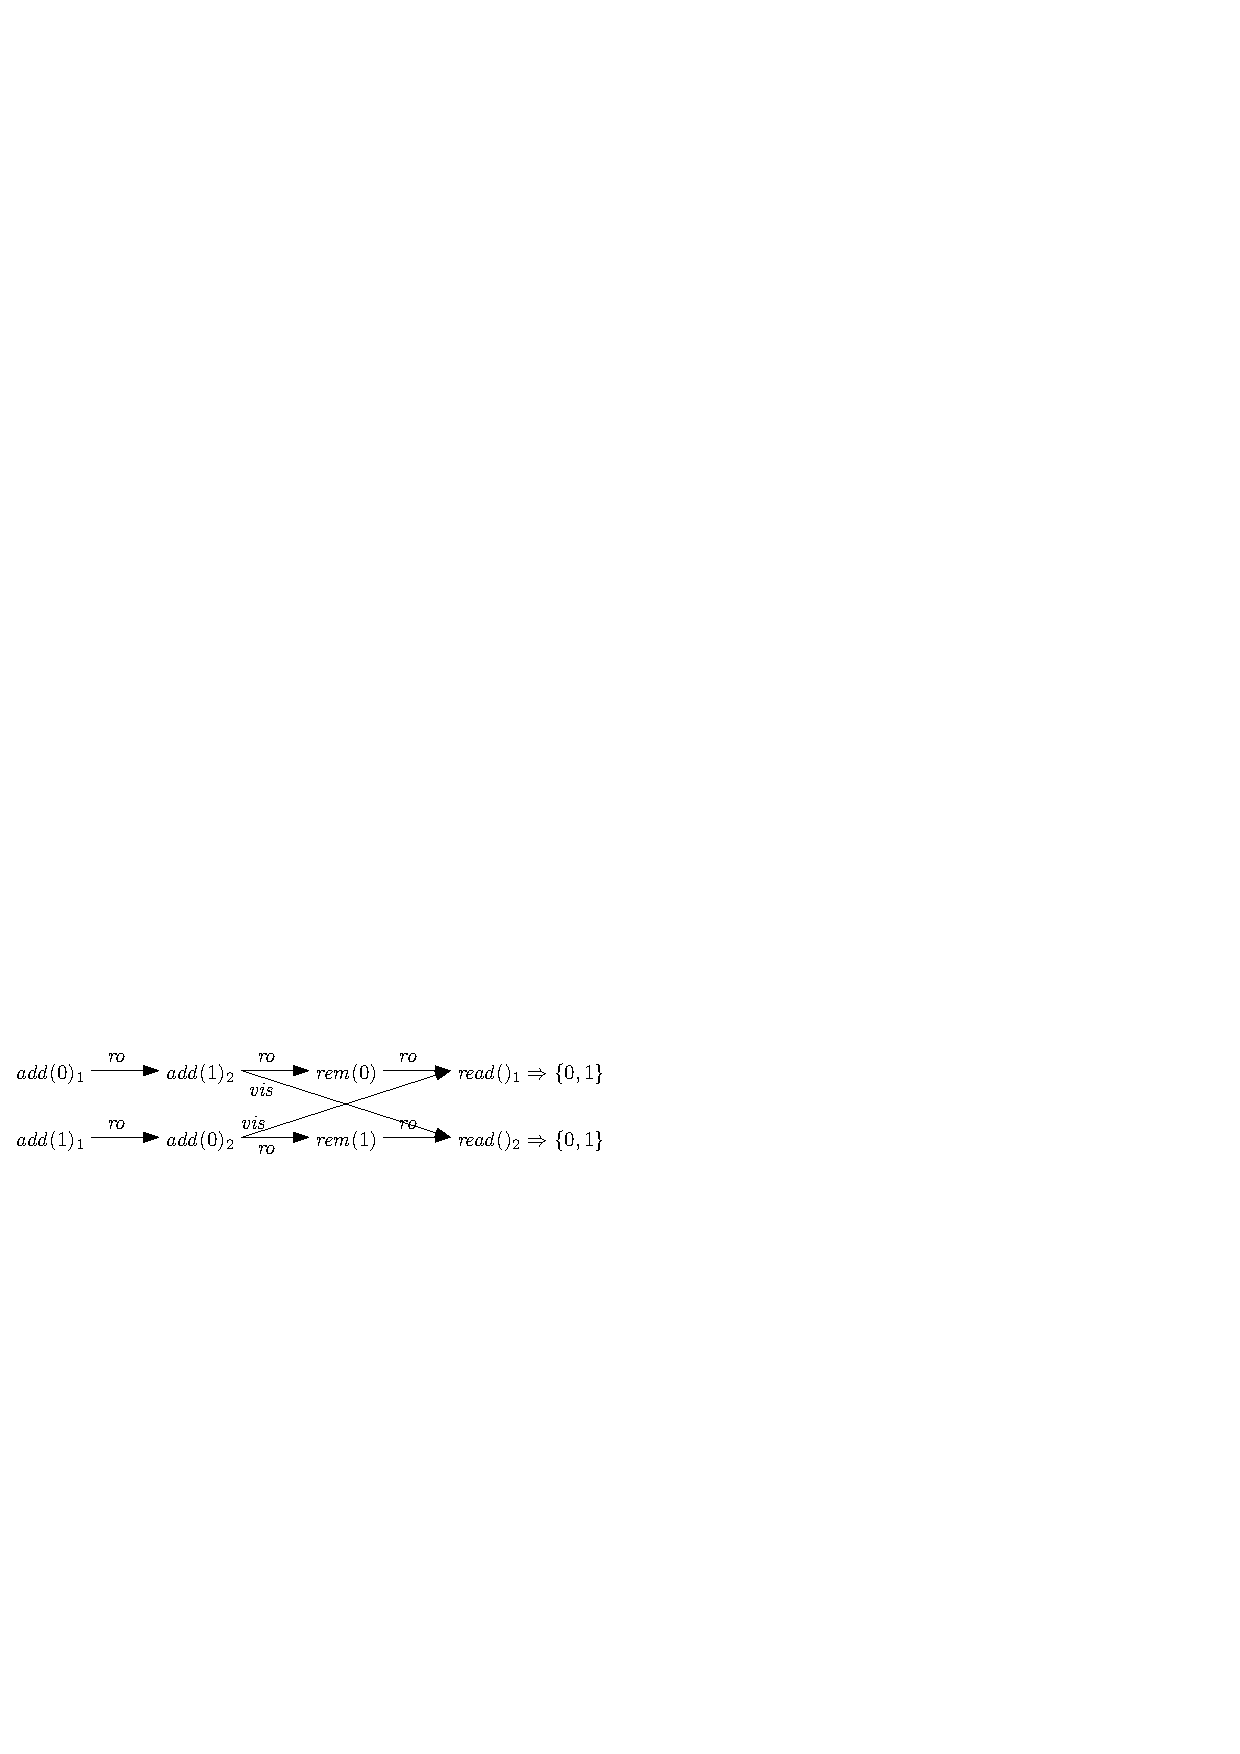
\includegraphics[width=0.7 \textwidth]{figures/PIC-Example-LinHis.pdf}
%\vspace{-10pt}
  \caption{A distributed linearizable history. Here subscript of $\mathit{add}(0)_1$ is used to distinguish different $\mathit{add}(0)$ operations.}
  \label{fig:a distributed linearizable history}
\end{figure}



\begin{figure}[t]
  \centering
  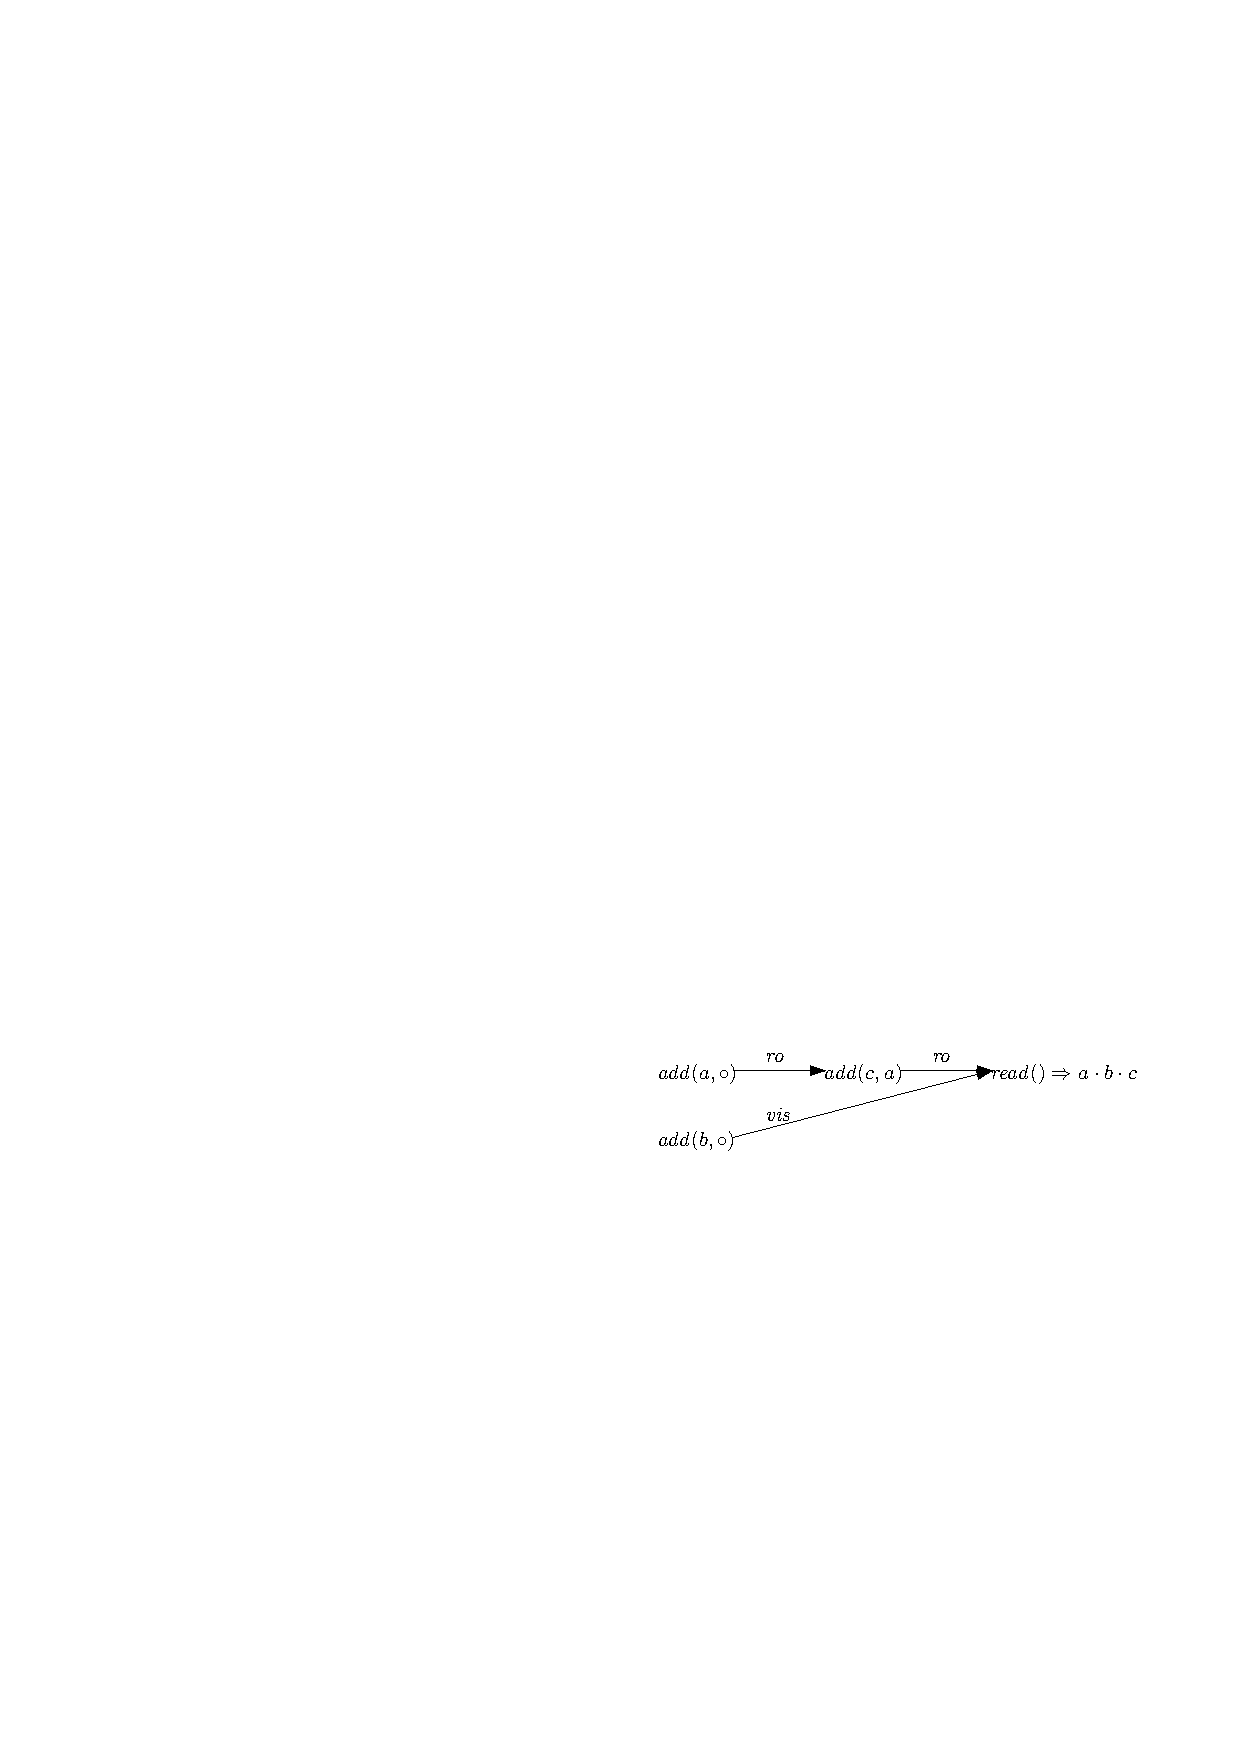
\includegraphics[width=0.6 \textwidth]{figures/PIC-Example-NonLinHis.pdf}
%\vspace{-10pt}
  \caption{A non-distributed linearizable history.}
  \label{fig:a non-distributed linearizable history}
\end{figure}






%%% Local Variables:
%%% mode: latex
%%% TeX-master: "draft"
%%% End:
